% This is the "preamble" of the document. This is where the format options get set.
% Pro-tip: things following the % mark will not be compiled by LaTeX. I'll be using them extensively to explain things as we go.
% Note: not to scare you off of LaTeX, but it's normal to have problems. And ya girl has been having some. I've included the copyright info at the bottom of the document from the guy who wrote this package, because his documentation doesn't entirely match how it's actually used. So this is a combination of his working preamble along with my added commentary or explanation. 
%% 


\documentclass[stu,12pt,floatsintext]{apa7}
% Document class input explanation ________________
% LaTeX files need to start with the document class, so it knows what it's using
% - This file is using the apa7 document class, as it has a lot of the formatting built in
% There are two sets of brackets in LaTeX, for each command (the things that start with the slash \ )
% - The squiggle brackets {} are mandatory for executing the command
% - The square brackets [] are options for that command. There can be more than one set of square brackets for some commands
% Options used in this document (general note - for each of these, if you want to use the other options, swap it out in that spot in the square brackets):
% - stu: this sets the `document mode' as the "student paper" version. Other options are jou (journal), man (manuscript, for journal submission), and doc (a plain document)
% --- The student setting includes things like 'duedate', 'course', and 'professor' on the title page. If these aren't wanted/needed, use the 'man' setting. It also defaults to including the tables and figures at the end of the document. This can be changed by including the 'floatsintext' option, as I have for you. If the instructor wants those at the end, remove that from the square brackets.
% --- The manuscript setting is roughly what you would use to submit to a journal, so uses 'date' instead of 'duedate', and doesn't include the 'course' or 'professor' info. As with 'stu', it defaults to putting the tables and figures at the end rather than in text. The same option will bump those images in text.
% --- Journal ('jou') outputs something similar to a common journal format - double columned text and figurs in place. This can be fun, especially if you are sumbitting this as a writing sample in applications.
% --- Document ('doc') outputs single columned, single spaced text with figures in place. Another option for producing a more polished looking document as a writing sample.
% - 12pt: sets the font size to 12pt. Other options are 10pt or 11pt
% - floatsintext: makes it so tables and figures will appear in text rather than at the end. Unforunately, not having this option set breaks the whole document, and I haven't been able to figure out why. IT's GREAT WHEN THINGS WORK LIKE THEY'RE SUPPOSED TO.

\usepackage[american]{babel}

\usepackage{csquotes} % One of the things you learn about LaTeX is at some level, it's like magic. The references weren't printing as they should without this line, and the guy who wrote the package included it, so here it is. Because LaTeX reasons.
\usepackage[style=apa,sortcites=true,sorting=nyt,backend=biber]{biblatex}
% biblatex: loads the package that will handle the bibliographic info. Other option is natbib, which allows for more customization
% - style=apa: sets the reference format to use apa (albeit the 6th edition)
\DeclareLanguageMapping{american}{american-apa} % Gotta make sure we're patriotic up in here. Seriously, though, there can be local variants to how citations are handled, this sets it to the American idiosyncrasies 
\addbibresource{bibliography.bib} % This is the companion file to the main one you're writing. It contains all of the bibliographic info for your references. It's a little bit of a pain to get used to, but once you do, it's the best. Especially if you recycle references between papers. You only have to get the pieces in the holes once.`

\usepackage[T1]{fontenc} 
\usepackage{mathptmx} % This is the Times New Roman font, which was the norm back in my day. If you'd like to use a different font, the options are laid out here: https://www.overleaf.com/learn/latex/Font_typefaces
% Alternately, you can comment out or delete these two commands and just use the Overleaf default font. So many choices!


% Title page stuff _____________________
\title{3D Model Reconstruction Using Laser Scanning} % The big, long version of the title for the title page
\shorttitle{} % The short title for the header
\author{Jule Valendo Halim - 1425567}
% \date{January 17, 2024} The student version doesn't use the \date command, for whatever reason
\affiliation{University of Melbourne}
\course{GEOM90038 Advanced Imaging} % LaTeX gets annoyed (i.e., throws a grumble-error) if this is blank, so I put something here. However, if your instructor will mark you off for this being on the title page, you can leave this entry blank (delete the PSY 4321, but leave the command), and just make peace with the error that will happen. It won't break the document.
\duedate{}
\professor{}  % Same situation as for the course info. Some instructors want this, some absolutely don't and will take off points. So do what you gotta.

%\keywords{APA style, demonstration} % If you need to have keywords for your paper, delete the % at the start of this line

\begin{document}
\maketitle % This tells LaTeX to make the title page

% \section{Introduction} This command is commented out, because I was taught it was redundant to have the paper's title and introduction together. If your instructor wants it to say "Introduction", delete the % at the start

Introductory text goes here. A wild example parenthetical reference appears \parencite{Contributor2023}, followed by an in-text sample citation by \textcite{FullBook2021}.

Note that paragraphs are separated by a blank line in the editor. If you do not do this, it will continue as a single paragraph.
This line is \textit{technically} on a new line in the editor, but will print in the same paragraph. \cite{Contributor2023}

\section{Introduction}

\section{Methodology}

\section{Results}

Statistical words. A demonstrative Figure~\ref{fig:OverallEffect}.

\begin{figure}
    \centering
    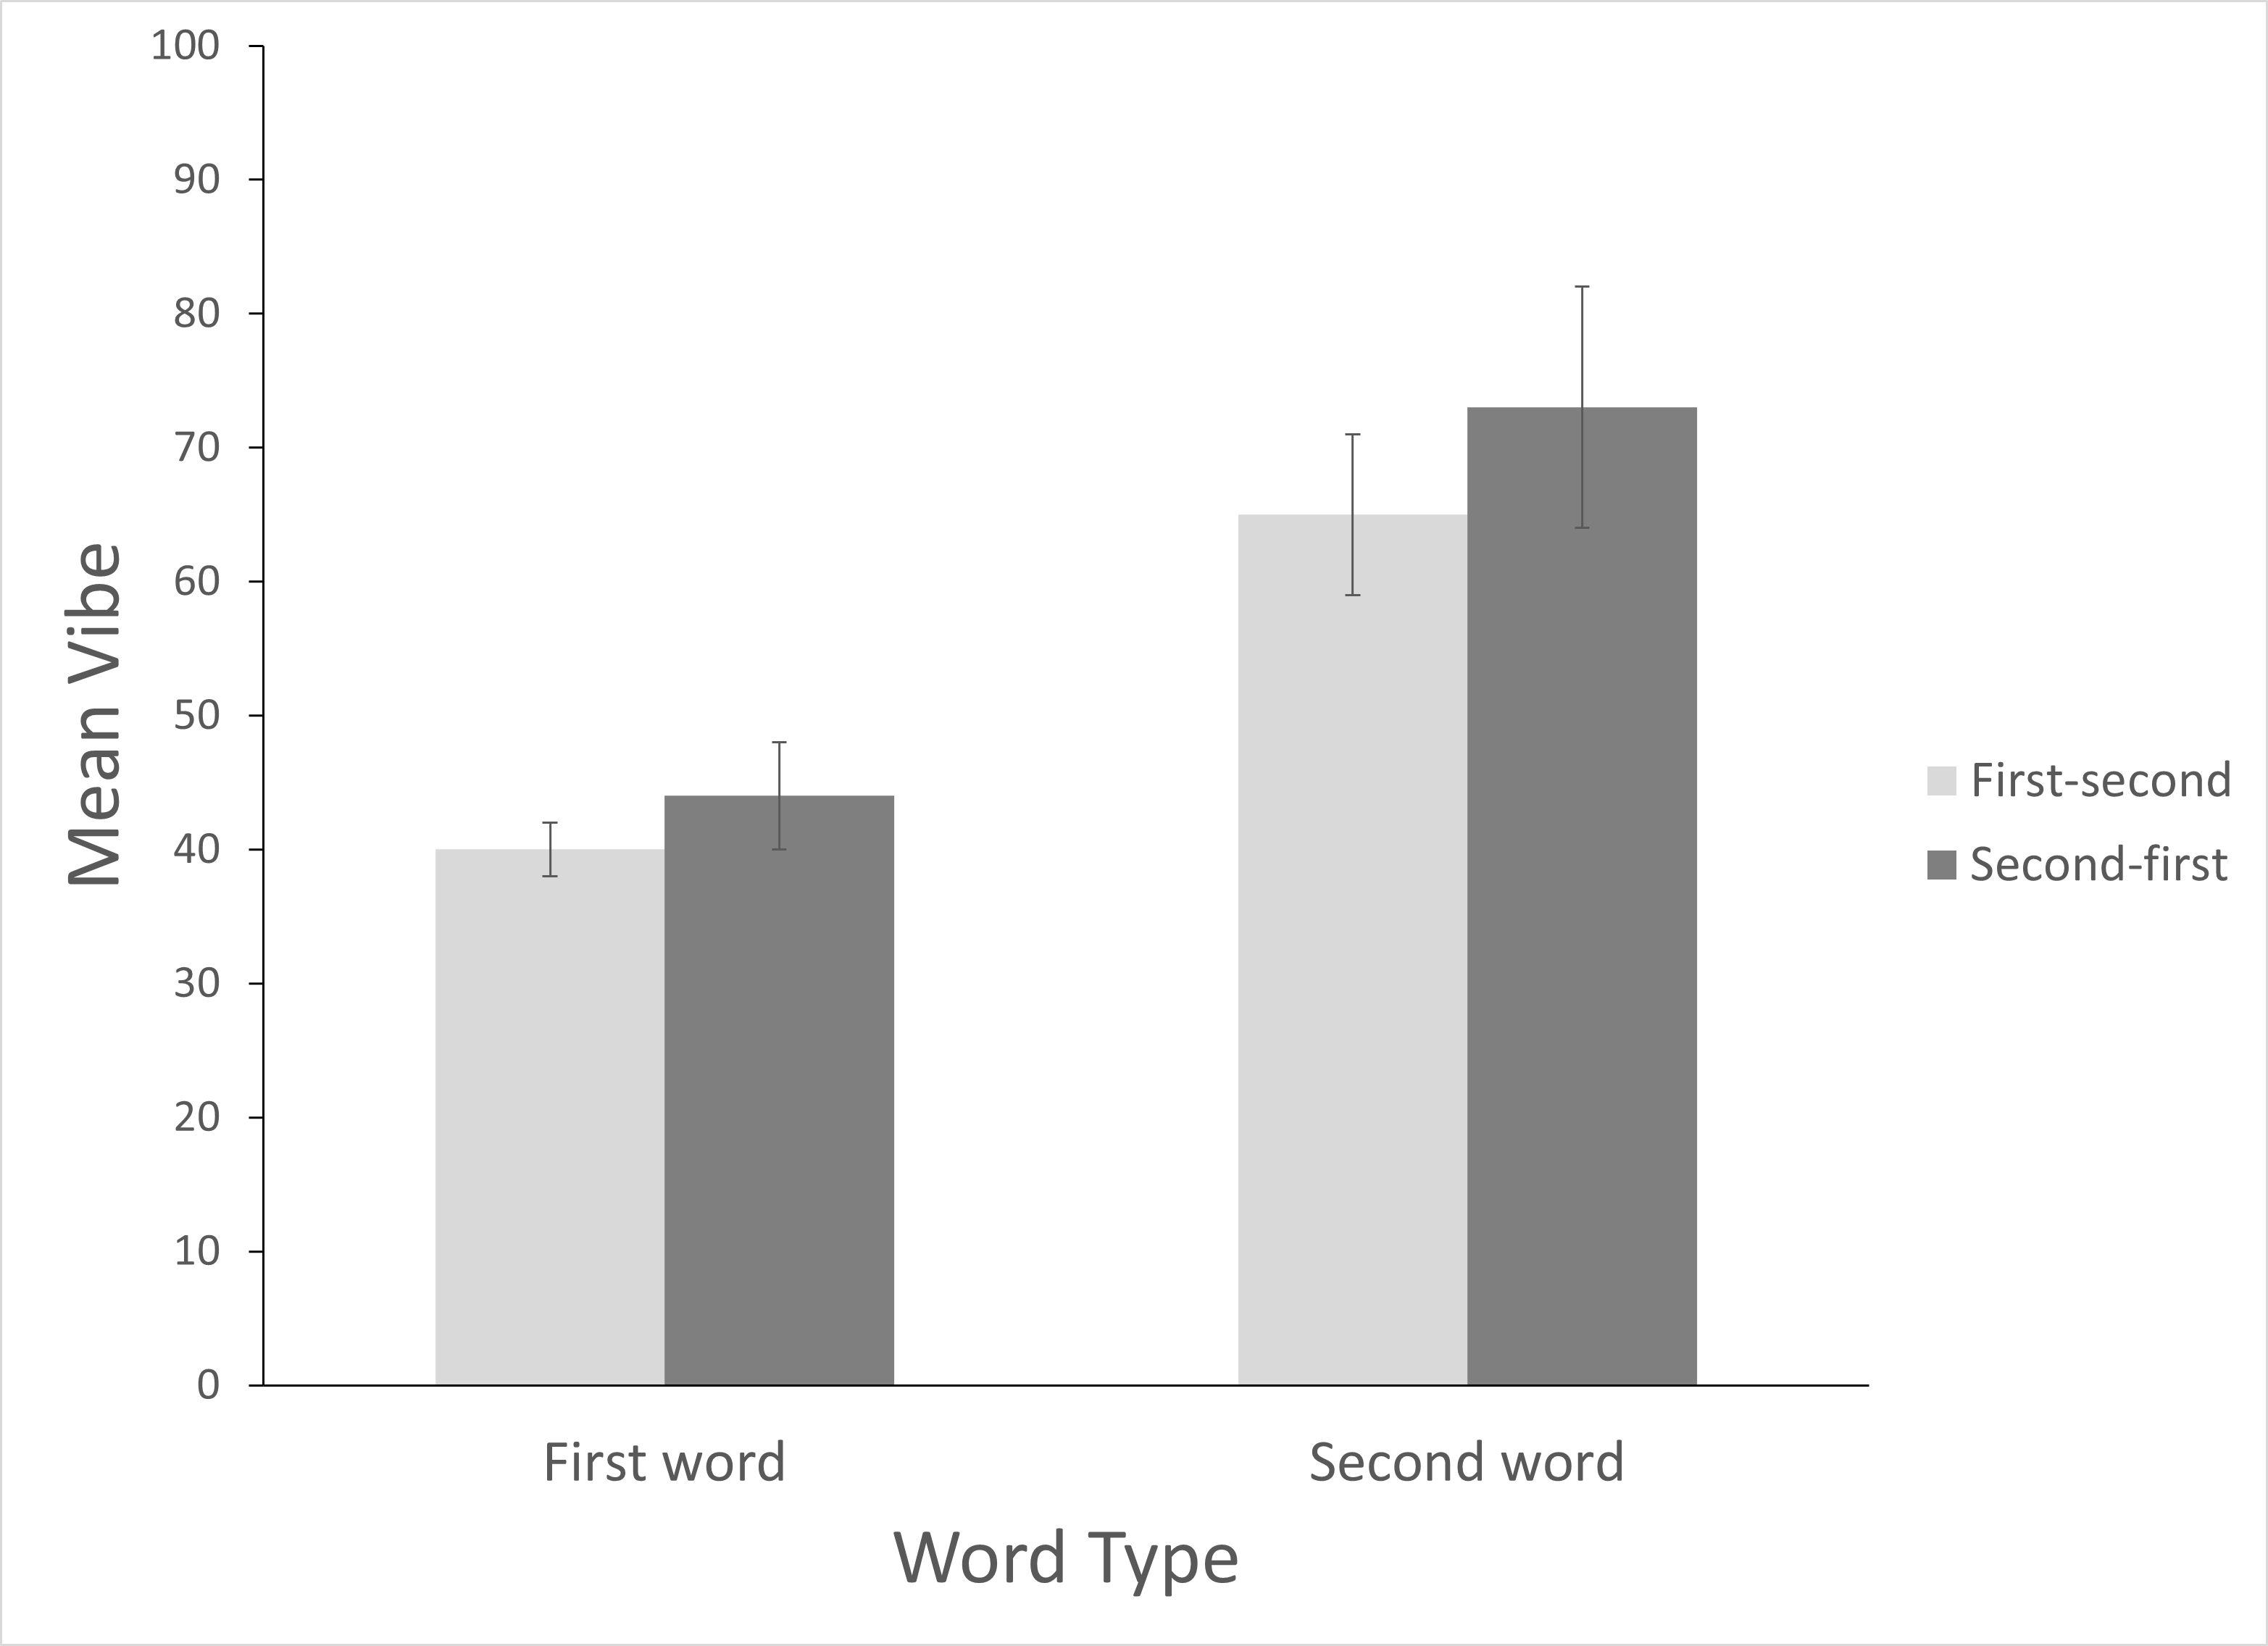
\includegraphics[width=0.75\linewidth]{sampleFig.png} % This is setting the figure to be .75x the width of the line. This can go all the way from 0.1 to 1 (and beyond, but then you're outside the page).
    \caption{The mean vibes for each word type and counterbalanced condition order. Error bars represent one standard error of the mean.}
    \label{fig:OverallEffect}
\end{figure}

\section{Conclusions and Discussions}

Discussion words.

\printbibliography

\end{document}

%% 
%% Copyright (C) 2019 by Daniel A. Weiss <daniel.weiss.led at gmail.com>
%% 
%% This work may be distributed and/or modified under the
%% conditions of the LaTeX Project Public License (LPPL), either
%% version 1.3c of this license or (at your option) any later
%% version.  The latest version of this license is in the file:
%% 
%% http://www.latex-project.org/lppl.txt
%% 
%% Users may freely modify these files without permission, as long as the
%% copyright line and this statement are maintained intact.
%% 
%% This work is not endorsed by, affiliated with, or probably even known
%% by, the American Psychological Association.
%% 
%% This work is "maintained" (as per LPPL maintenance status) by
%% Daniel A. Weiss.
%% 
%% This work consists of the file  apa7.dtx
%% and the derived files           apa7.ins,
%%                                 apa7.cls,
%%                                 apa7.pdf,
%%                                 README,
%%                                 APA7american.txt,
%%                                 APA7british.txt,
%%                                 APA7dutch.txt,
%%                                 APA7english.txt,
%%                                 APA7german.txt,
%%                                 APA7ngerman.txt,
%%                                 APA7greek.txt,
%%                                 APA7czech.txt,
%%                                 APA7turkish.txt,
%%                                 APA7endfloat.cfg,
%%                                 Figure1.pdf,
%%                                 shortsample.tex,
%%                                 longsample.tex, and
%%                                 bibliography.bib.
%% 
%%
%%
%% This is file `./samples/shortsample.tex',
%% generated with the docstrip utility.
%%
%% The original source files were:
%%
%% apa7.dtx  (with options: `shortsample')
%% ----------------------------------------------------------------------
%% 
%% apa7 - A LaTeX class for formatting documents in compliance with the
%% American Psychological Association's Publication Manual, 7th edition
%% 
%% Copyright (C) 2019 by Daniel A. Weiss <daniel.weiss.led at gmail.com>
%% 
%% This work may be distributed and/or modified under the
%% conditions of the LaTeX Project Public License (LPPL), either
%% version 1.3c of this license or (at your option) any later
%% version.  The latest version of this license is in the file:
%% 
%% http://www.latex-project.org/lppl.txt
%% 
%% Users may freely modify these files without permission, as long as the
%% copyright line and this statement are maintained intact.
%% 
%% This work is not endorsed by, affiliated with, or probably even known
%% by, the American Psychological Association.
%% 
%% ----------------------------------------------------------------------